\chapter{Implementation}
This chapter discuss the implementation of the different architectural parts of the approach, which are outlined in the chapter before.

\label{ch:implementation}
\section{Middleware}
As stated in the architectural overview, a middleware shall be provided that devices can use to communicate with each other and exchange run-time states. In this prototypical implementation, we used MQTT Protocol and Eclipse Mosquitto™\footnote{\url{https://mosquitto.org/}} which is a MQTT-based message broker.

\subsection{MQTT}
MQTT is a lightweight messaging protocol for the Internet of Things (IoT). As it allows connecting a large number of devices and bi-directional communications, it is ideal for being a message broker in a publish/subscribe infrastructure. The protocol supports a variety of popular programming languages and platforms\cite{mqtt}. MQTT is lightweight and optimizes network bandwidth because of small message headers. Many devices rely on unreliable cellular networks to communicate. The support for persistent sessions in MQTT reduces the time it takes for the client to reconnect with the message broker.

We use an open-source MQTT broker, Eclipse Mosquitto™, which offers a MQTT server and client implementations that are compliant with relevant standards.
\cite{mosquitto}

\subsection{Server Specifications}
We installed Mosquitto on a VPS with Ubuntu 18.02 operating system to have a running MQTT broker. This VPS has a public IP address so that devices can connect over the internet as clients. The hardware specification of this VPS is 1 CPU, 1GB RAM, and 20GB SDD. 

\section{Deriving Interfaces}
Developers should derive interfaces from Application State Models. These interfaces must be written in the programming language of source and target applications. Developers should write a glue code to connect the source code of the existing application and use Application State Models' interfaces. These interfaces should be used as a type for a run-time state, and they guarantee these values. These interfaces can be written by developers or get generated with ASML CLI, a helper tool explained in 7.5.3.

\section{Libraries}
Two libraries are developed in two different popular programming languages, which are JavaScript and Java. These libraries are using the native API of their platform (Desktop and Android) to help developers implement run-time state migration. Each library is using a client library for MQTT Protocol to manage the communication with other devices. Developers must write some glue code to integrate libraries into existing applications. Figure \ref{fig:libraries-component} shows the component diagram of the library. The \textit{ASML Schema} is used by \textit{Validator} to validate a run-time state. The \textit{Library API} is the implementation of API Reference which can communicate with MQTT Library. The \textit{MQTT Library} can publish messages via \textit{Middleware}. Moreover, developers can write glue code and call methods of the library via \textit{Library API}.

\FloatBarrier
\begin{figure}[H]
    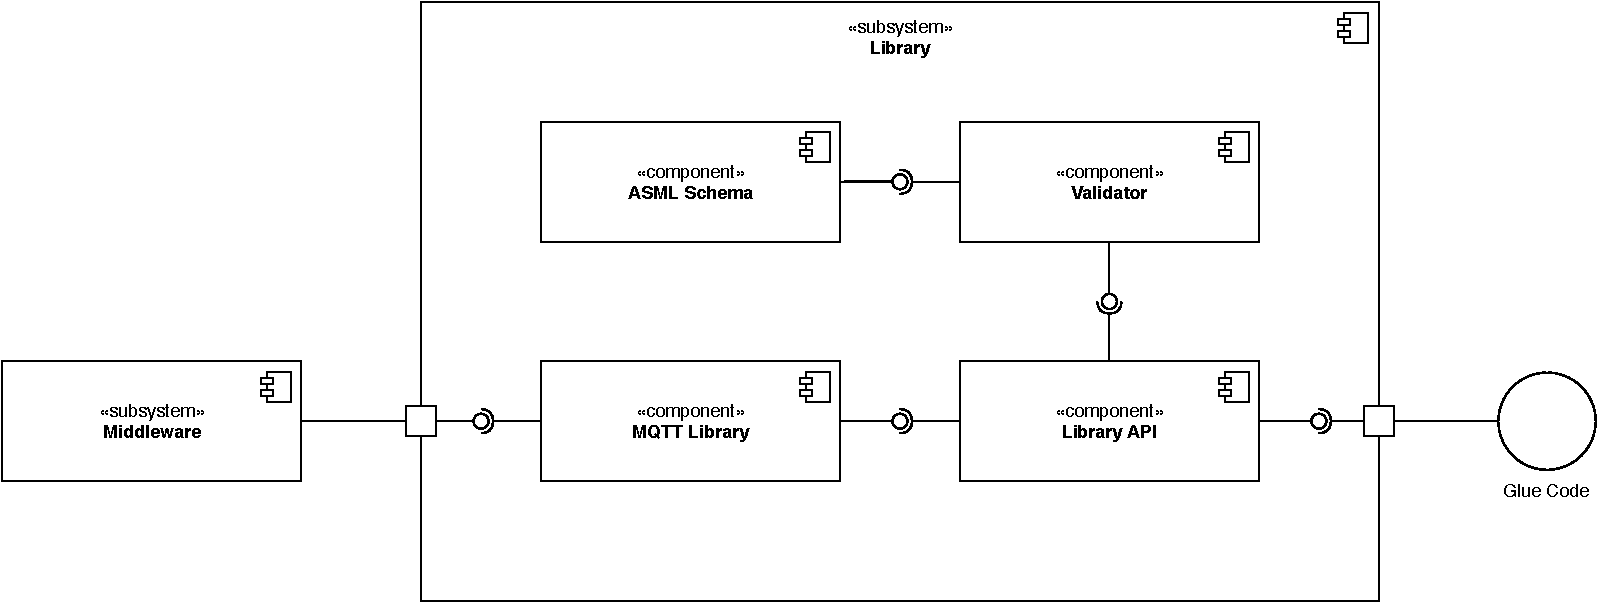
\includegraphics[width=0.8\textwidth]{../figures/libraries-diagram.pdf}
    \centering
    \caption{The component diagram of the library}
    \label{fig:libraries-component}
\end{figure}
\FloatBarrier

\subsection{API Reference}
In the following, the reference API for the library is provided. This reference API is support by the two existing implementation for JavaScript and Java. Also, if other developers want to support other programming languages, they can follow this API Reference. 

\subsubsection{addModel}
Each Application State Model must be added to the library. This method allows developers to add a valid Application State Model's support by adding its interface as an input parameter.

\subsubsection{getModel}
This method allows retrieving the added Application State Model by its name.

\subsubsection{getModels}
This method allows retrieving all Application State Models that the device is supporting. 

\subsubsection{introduce}
An application should introduce itself to other applications on the network via middleware. In this method, configuration parameters must be provided. These parameters are device identification, device and application name, middleware IP address, and a value that shows if it is a new device. The library should generate a unique device identification like UUID. This method subscribes the device to the online topic, and all topics of supported Application State Models, then publish configuration parameters as a message in JSON format via MQTT Protocol to corresponding topics. The middleware forwards the message to all devices that support the same Application State Model. A callback \textit{onDeviceJoin} which explained in 7.3.2, will be called on all recipients of a introduction message and they should add the new device to their devices list. Also, they responds with a introduction message but only to the new device. Thereby, the new device adds other devices to the devices list. For instance, Application State Models, which Mailspring supports, are \textit{search} and \textit{sending-email}. Also, K-9 Mail supports \textit{search} and \textit{sending-email} as well. Listing \ref{lis:api-introduction-source} shows the introduction of Mailspring published to all devices which support \textit{search} and \textit{sending-email}.

As each application and platform has different life cycle and entry points, calling this method is part of the glue code and needs to be coupled with the application. So, when an application starts, this method should be called.

\FloatBarrier
\begin{code}
\begin{js2}
// topics:
// search
// sending-email
\end{js2}
\begin{json}
{
   "action":"device",
   "data":{
      "device":{
         "id":"35fe23c2-bf7c-4988-b934-46f7ba12a807",
         "name":"Mailspring - macOS"
      },
      "new":true
   }
}
\end{json}
\caption{The device introduction message.}
\label{lis:api-introduction-source}
\end{code}
\FloatBarrier


Also, Listing \ref{lis:api-introduction-target} shows K-9 Mail introduction respond which  published to Mailspring's \textit{search} and \textit{sending-email} topics.

\FloatBarrier
\begin{code}
\begin{js2}
// topics:
// search/35fe23c2-bf7c-4988-b934-46f7ba12a807
// sending-email/35fe23c2-bf7c-4988-b934-46f7ba12a807
\end{js2}

\begin{json}
{
   "action":"device",
   "data":{
      "device":{
         "id":"46f7ba12a807-bf7c-4988-b934-35fe23c2",
         "name":"K-9 Mail - Android"
      }
   }
}
\end{json}
\caption{The device introduction respond message.}
\label{lis:api-introduction-target}
\end{code}
\FloatBarrier


\subsubsection{getDevice}
This method allows fetching the configuration parameters of the current device. These parameters should set by the introduction method.

\subsubsection{setState}
Developers needs to extract the run-time state and adjusted it to corresponding interface.
To keep track of run-time time state and extract it, different events might occurs on changing a run-time state on different programming languages (e.g onClick or onChange).
This method allows developers store the current run-time state after adjustment in the library. If a device requests a run-time state, it is ready to get migrated. 

\subsubsection{setHasState}
A device must have a run-time state to migrate. This method notifies other devices about having a run-time state for a particular Application State Model. This method sends a message in JSON format via MQTT Procotol to all supported Application State Models topics and inform them whether this device has a state or not. Other devices should add or remove this device in the list of their devices based on the value in the message. For instance, as mentioned before Mailspring supports \textit{search} and \textit{sending-email}, Listing \ref{lis:api-sethasstate} shows Mailpsring publish a message to corresponding topics.


\FloatBarrier
\begin{code}
\begin{js2}
// topics:
// search
// sending-email
\end{js2}

\begin{json}
{
   "action":"has-state",
   "data":{
      "device":{
         "_id":"35fe23c2-bf7c-4988-b934-46f7ba12a807",
         "name":"Mailspring - macOS"
      },
      "value":true
   }
}
\end{json}
\caption{Mailspring informs other devices that has a run-time state.}
\label{lis:api-sethasstate}
\end{code}
\FloatBarrier


\subsubsection{getDevices}
For run-time state migration, the target device must be known and get selected. A list of devices that support common Application State Models should be stored in the library. This method allows fetching all devices for a particular Application State Model. Moreover, it should be distinguishable if a device has a run-time state or it only supports the same Application State Model.

\subsubsection{getStateDevice}
After the target device got chosen from \textit{getDevices} method, the source device can request its run-time state. This method allows the get a run-time state of a particular Application State Model from a particular device. This method should send a message in JSON format via MQTT Protocol to a device from which a state shall be retrieved and request its run-time state. Listing \ref{lis:api-getstate} shows an example in which Mailspring requests a run-time state of \textit{search} Application State Model from K-9 Mail by publishing a message to the corresponding topic.

\FloatBarrier
\begin{code}
\begin{js2}
// topic:
// search/46f7ba12a807-bf7c-4988-b934-35fe23c2
\end{js2}

\begin{json}
{
   "action":"request-state",
   "data":{
      "device":{
         "_id":"35fe23c2-bf7c-4988-b934-46f7ba12a807",
         "name":"Mailspring - macOS"
      }
   }
}
\end{json}
\caption{Mailspring request a run-time state from K-9 Mail.}
\label{lis:api-getstate}
\end{code}
\FloatBarrier

\subsubsection{sendState}
This method allows devices to send a particular run-time state to a particular device. This migration process can be the push method, which sends the run-time state directly to a target device, or the pull method, which response to the request of \textit{getStateDevice} method. Listing \ref{lis:api-sendstate} shows K-9 Mail sends the run-time state of \textit{search} Application State Model to Mailspring by publishing a message to the corresponding topic.


\FloatBarrier
\begin{code}
\begin{js2}
// topic:
// search/35fe23c2-bf7c-4988-b934-46f7ba12a807
\end{js2}

\begin{json}
{
   "action":"response-state",
   "data":{
      "device":{
         "_id":"46f7ba12a807-bf7c-4988-b934-35fe23c2",
         "name":"K-9 Mail - Android"
      },
      "state":{
         "query":"this is a test",
         "submit":true
      }
   }
}
\end{json}
\caption{K-9 Mail sends run-time state of \textit{search} to Mailspring.}
\label{lis:api-sendstate}
\end{code}
\FloatBarrier

\subsubsection{setMigration}
This method allows the target device to notify the source device about finalizing the run-time state migration process. This method should be called when the target application adjusted the new run-time time state to its UI. This method should send a message in JSON format via MQTT Protocol to the source device and inform the end of migration. Also, the source application should react upon receiving this message by removing its run-time state. For instance, if a e-mail draft is migrated, this drafted can be closed on the source device. Listing \ref{lis:api-sendstate} shows Mailspring sends the migration message of \textit{search} Application State Model to K-9 Mail by publishing a message to the corresponding topic.

\FloatBarrier
\begin{code}
\begin{js2}
// topic:
// search/46f7ba12a807-bf7c-4988-b934-35fe23c2
\end{js2}

\begin{json}
{
   "action":"migration",
   "data":{
      "device":{
         "_id":"35fe23c2-bf7c-4988-b934-46f7ba12a807",
         "name":"Mailspring - macOS"
      }
   }
}
\end{json}
\caption{K-9 Mail sends migration message to Mailspring.}
\label{lis:api-setmigration}
\end{code}
\FloatBarrier

\subsubsection{onMessage}
This method should be called on applications which receive a message from middleware. This method is responsible of message process and filtering and calling a corresponding callback. For instance, when a device receive a message with \mintinline{json}{{"action": "response-state"}} (Figure \ref{lis:api-sendstate}), this method calls the \textit{onStateReceive} callback, which explained in 7.3.2.


\subsubsection{onOnline}
This method should be called on applications which receive a message about connectivity status of other devices from middleware. This method process the online status. If the a device goes offline, this method calls \textit{onDeviceLeave} callback, which explained in 7.3.2.

\subsection{Callback Events}
Devices should get a notice when they received a message via middleware. The library is responsible for the process of selecting messages for reception and processing them by \textit{onMessage} method. There should be callback events that allow developers to implement a proper behavior. This implementation is part of the glue code.

\subsubsection{onStateRequest}
This event should be called on the target application when the source application requests a run-time state via \textit{getStateDevice} method.

\subsubsection{onStateReceive}
This event should be called on the source application when the target application sends a run-time state via \textit{sendState} method.

\subsubsection{onStateMigration}
This event should be called on the source application when the target application is finalized the run-time state migration via \textit{setMigration} method.

\subsubsection{onDeviceJoin}
This event should be called on any application when a device that supports the same Application State Models joins the network via \textit{introduction} method.

\subsubsection{onDeviceLeave}
This event should be called on any application when a device that supports the same Application State Models leaves the network.


\subsection{JavaScript Library}
In recent years JavaScript is one of the most popular programming languages and supports various platforms. Also, TypeScript is a programming language that is a superset of JavaScript and transcompiles to JavaScript  \cite{typescript}. In our approach, the API Reference methods are implemented in a JavaScript library. This library is written in TypeScript, which supports static typing. The library source code is available on GitHub\footnote{\url{https://github.com/asml-lang/rsm-node}} and published on NPM\footnote{\url{https://www.npmjs.com/package/rsm-node}}.

The JavaScript library is using \lstinline[basicstyle=\ttfamily]{MQTT.js} and \lstinline[basicstyle=\ttfamily]{async-mqtt} libraries to bring MQTT Protocol in our JavaScript library.


\subsection{Android Library}
As the run-time state migration approach is meant to be supported on different platforms, we implemented the API Reference methods in another library for Android to support mobile devices. This library is written in Java, and
the source code is available on GitHub\footnote{\url{https://github.com/asml-lang/rsm-android}}. Also, it is published on Bintray\footnote{\url{https://bintray.com/saman/maven/rsm-android}}.

The Android library is using \lstinline[basicstyle=\ttfamily]{paho-mqtt} library to bring MQTT Protocol in our Android library.

\section{Demo Applications (MVP)}
Two demo applications are developed as minimum viable products (MVP). The purpose of developing these applications is to test the state exchange and communication part of the approach without mixing it with the application logic of an existing application. Figure \ref{fig:mvp} shows the screenshot of these applications. A Desktop application\footnote{\url{https://github.com/asml-lang/rsm-demo}} which is develop by Electron and written in JavaScript and an Android application\footnote{\url{https://github.com/asml-lang/rsm-demo-android}} written in Java. Both applications are using the corresponding library.

\FloatBarrier
\begin{figure}[H]
    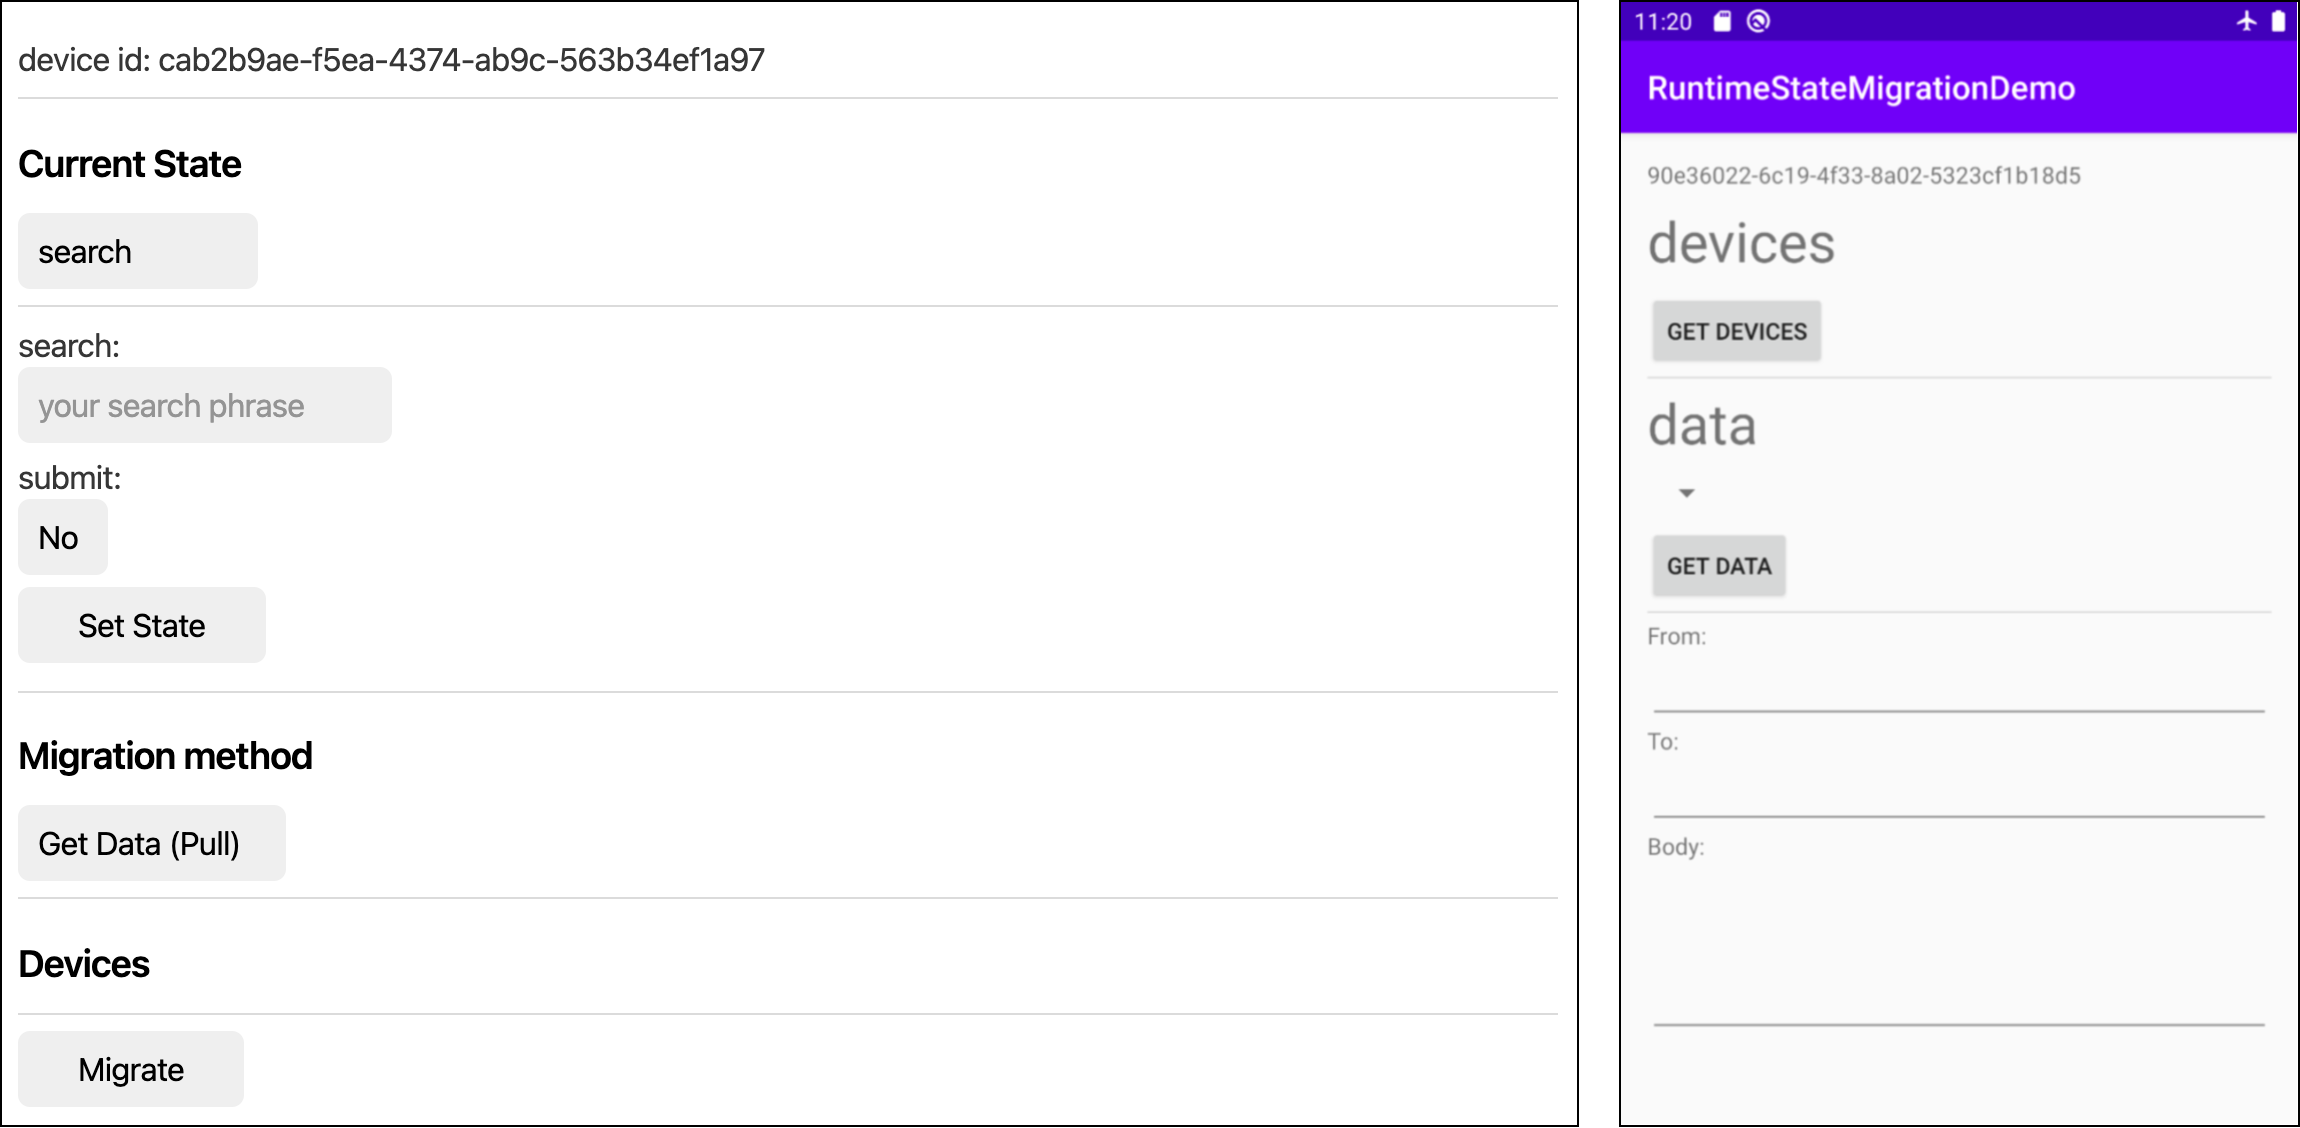
\includegraphics[width=\linewidth]{../figures/mvp.png}
    \centering
    \caption{Electron (Left) and Android (Right) MVP Applications}
    \label{fig:mvp}
\end{figure}
\FloatBarrier

% \section{Transferring Run-time State}
% \subsection{Initializing}
\begin{figure}
    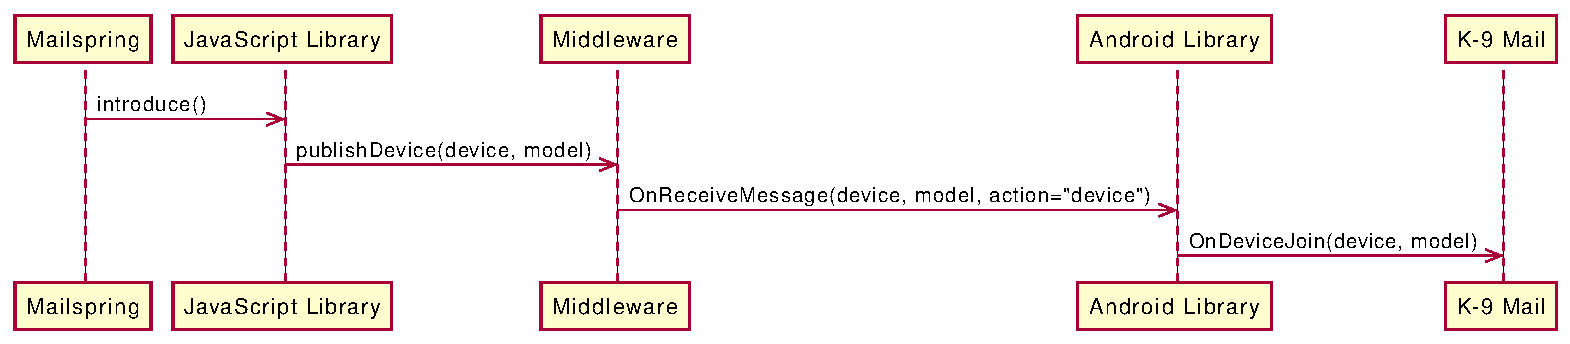
\includegraphics[width=\linewidth]{../figures/Initializing-Mailspring}
    \centering
    \caption{Initializing: Mailspring}
    \label{fig:Initializing-Mailspring}
\end{figure}

\subsection{Run-time State Management}
\subsubsection{Store State}
\begin{figure}
    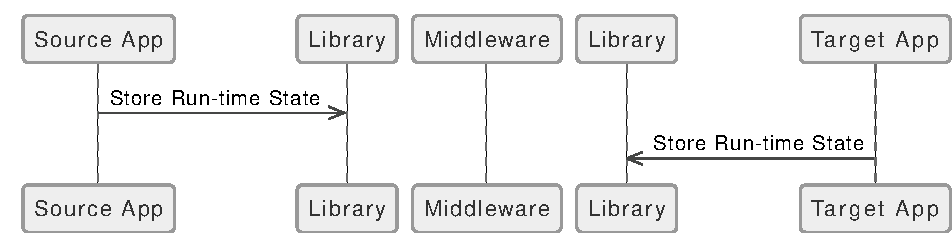
\includegraphics[width=\linewidth]{../figures/Store-Current-State}
    \centering
    \caption{Store the Current State}
    \label{fig:Store-Current-State}
\end{figure}
\subsubsection{Has State}
\begin{figure}
    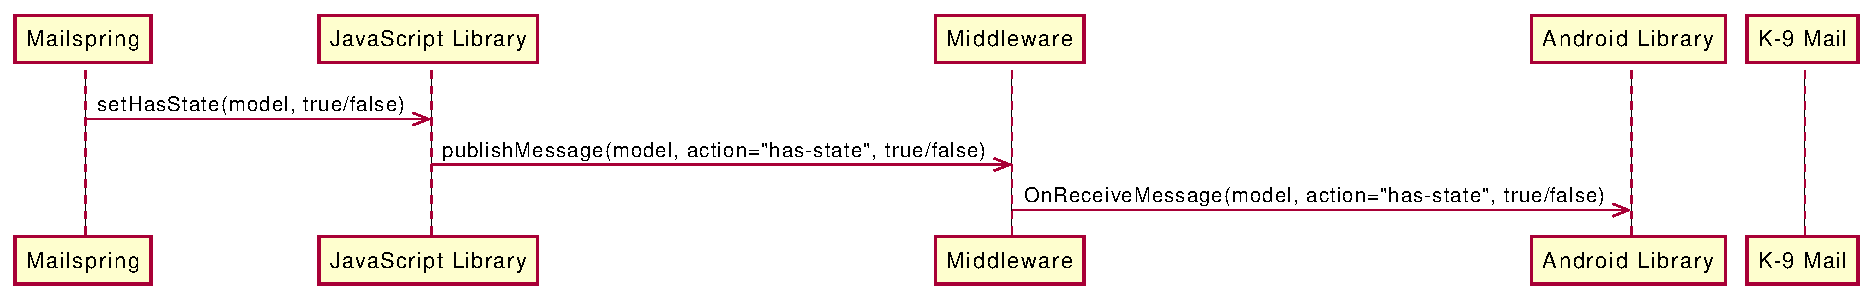
\includegraphics[width=\linewidth]{../figures/Inform-Devices-Has-State-Mailspring}
    \centering
    \caption{Inform other devices has a State: Mailspring}
    \label{fig:Inform-Devices-Has-State-Mailspring}
\end{figure}

\subsection{Migration Patterns}
\subsubsection{Pull Method}
\begin{figure}
    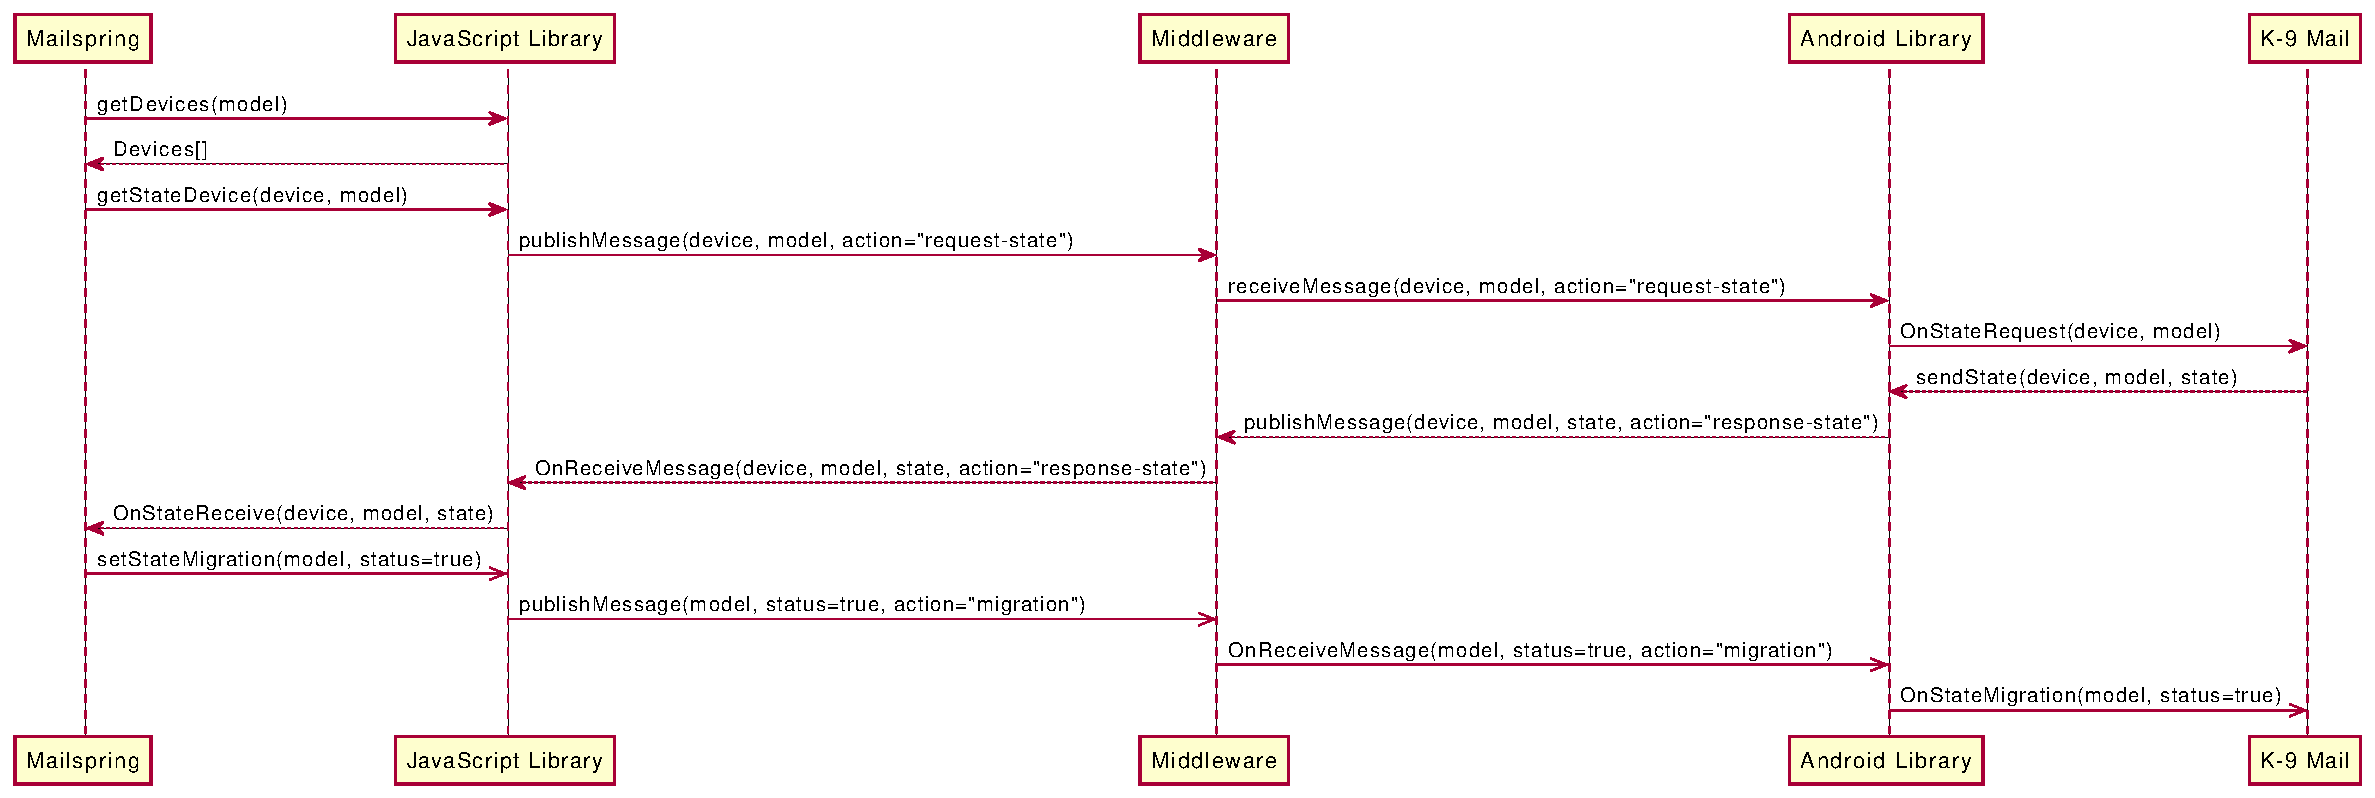
\includegraphics[width=\linewidth]{../figures/Migration-Mailspring-to-K9-Pull-Method}
    \centering
    \caption{Pull Method: Migration Mailspring to K9}
    \label{fig:Migration-Mailspring-to-K9-Pull-Method}
\end{figure}

\subsubsection{Push Method}
\begin{figure}
    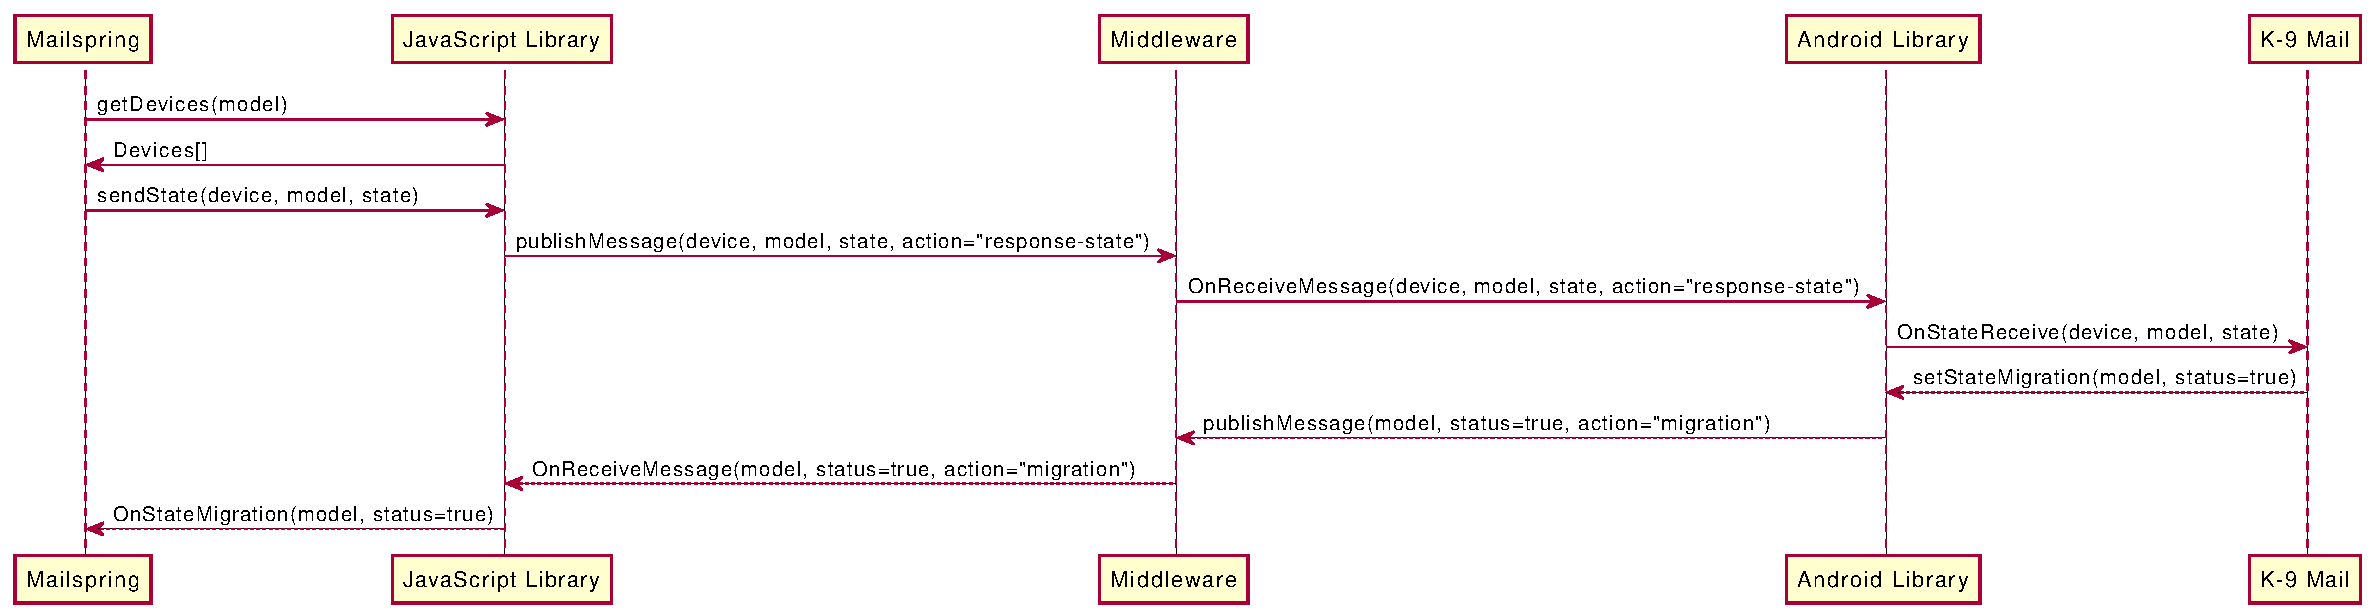
\includegraphics[width=\linewidth]{../figures/Migration-Mailspring-to-K9-Push-Method}
    \centering
    \caption{Push Method: Migration Mailspring to K9}
    \label{fig:Migration-Mailspring-to-K9-Push-Method}
\end{figure}

\subsection{Going Offline}
\subsubsection{Graceful}
\begin{figure}
    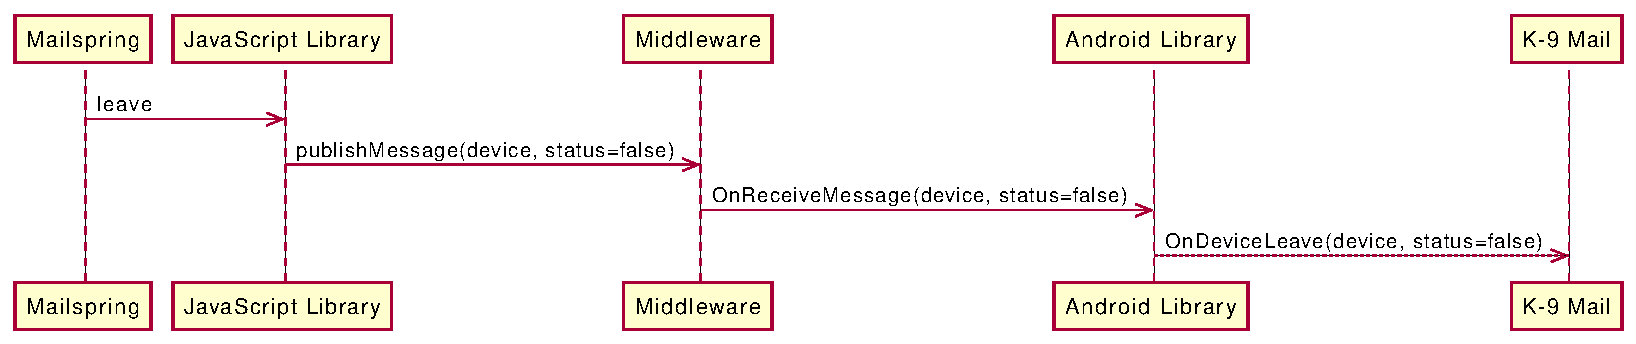
\includegraphics[width=\linewidth]{../figures/Going-Offline-Graceful-Mailspring}
    \centering
    \caption{Going Offline Gracefully: Mailspring}
    \label{fig:Going-Offline-Graceful-Mailspring}
\end{figure}
\subsubsection{Ungraceful}
\begin{figure}
    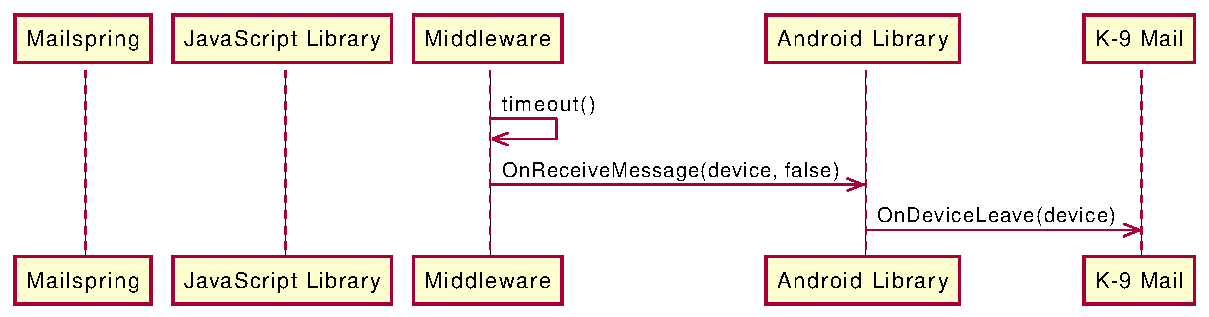
\includegraphics[width=\linewidth]{../figures/Going-Offline-Ungraceful-Mailspring}
    \centering
    \caption{Going Offline Ungracefully: Mailspring}
    \label{fig:Going-Offline-Ungraceful-Mailspring}
\end{figure}

\section{Helper Tools}
In the section, we explain some tools which are implemented to help developers. These tools are designed to increase code quality, reuse existing code, and reduce development time.
\subsection{ASML Schema Library}
A repository hosted on GitHub\footnote{\url{https://github.com/asml-lang/asml}} contains the latest version of Application State Modeling Language abstract syntax, which is JSON a Schema document. Also, this repository contains some examples and the DSL manual. Moreover, for ease of implementation, this repository is published on NPM\footnote{\url{https://www.npmjs.com/package/asml}}. Furthermore, other JavaScript packages in this thesis are using it as the main schema.
 

\subsection{ASML Editor}
ASML Editor is a playground web application\footnote{\url{https://asml-lang.github.io/asml/editor/}} developed in HTML,CSS, and JavaScript. ASML Editor's purpose is to assist developers in writing Application State Models and validate a Run-Time State against it. In case of a validation or syntax error in any section, an error box shows up below that section and displays the error description like in Figure \ref{fig:asml-editor}. 
\FloatBarrier \begin{figure}[H]
    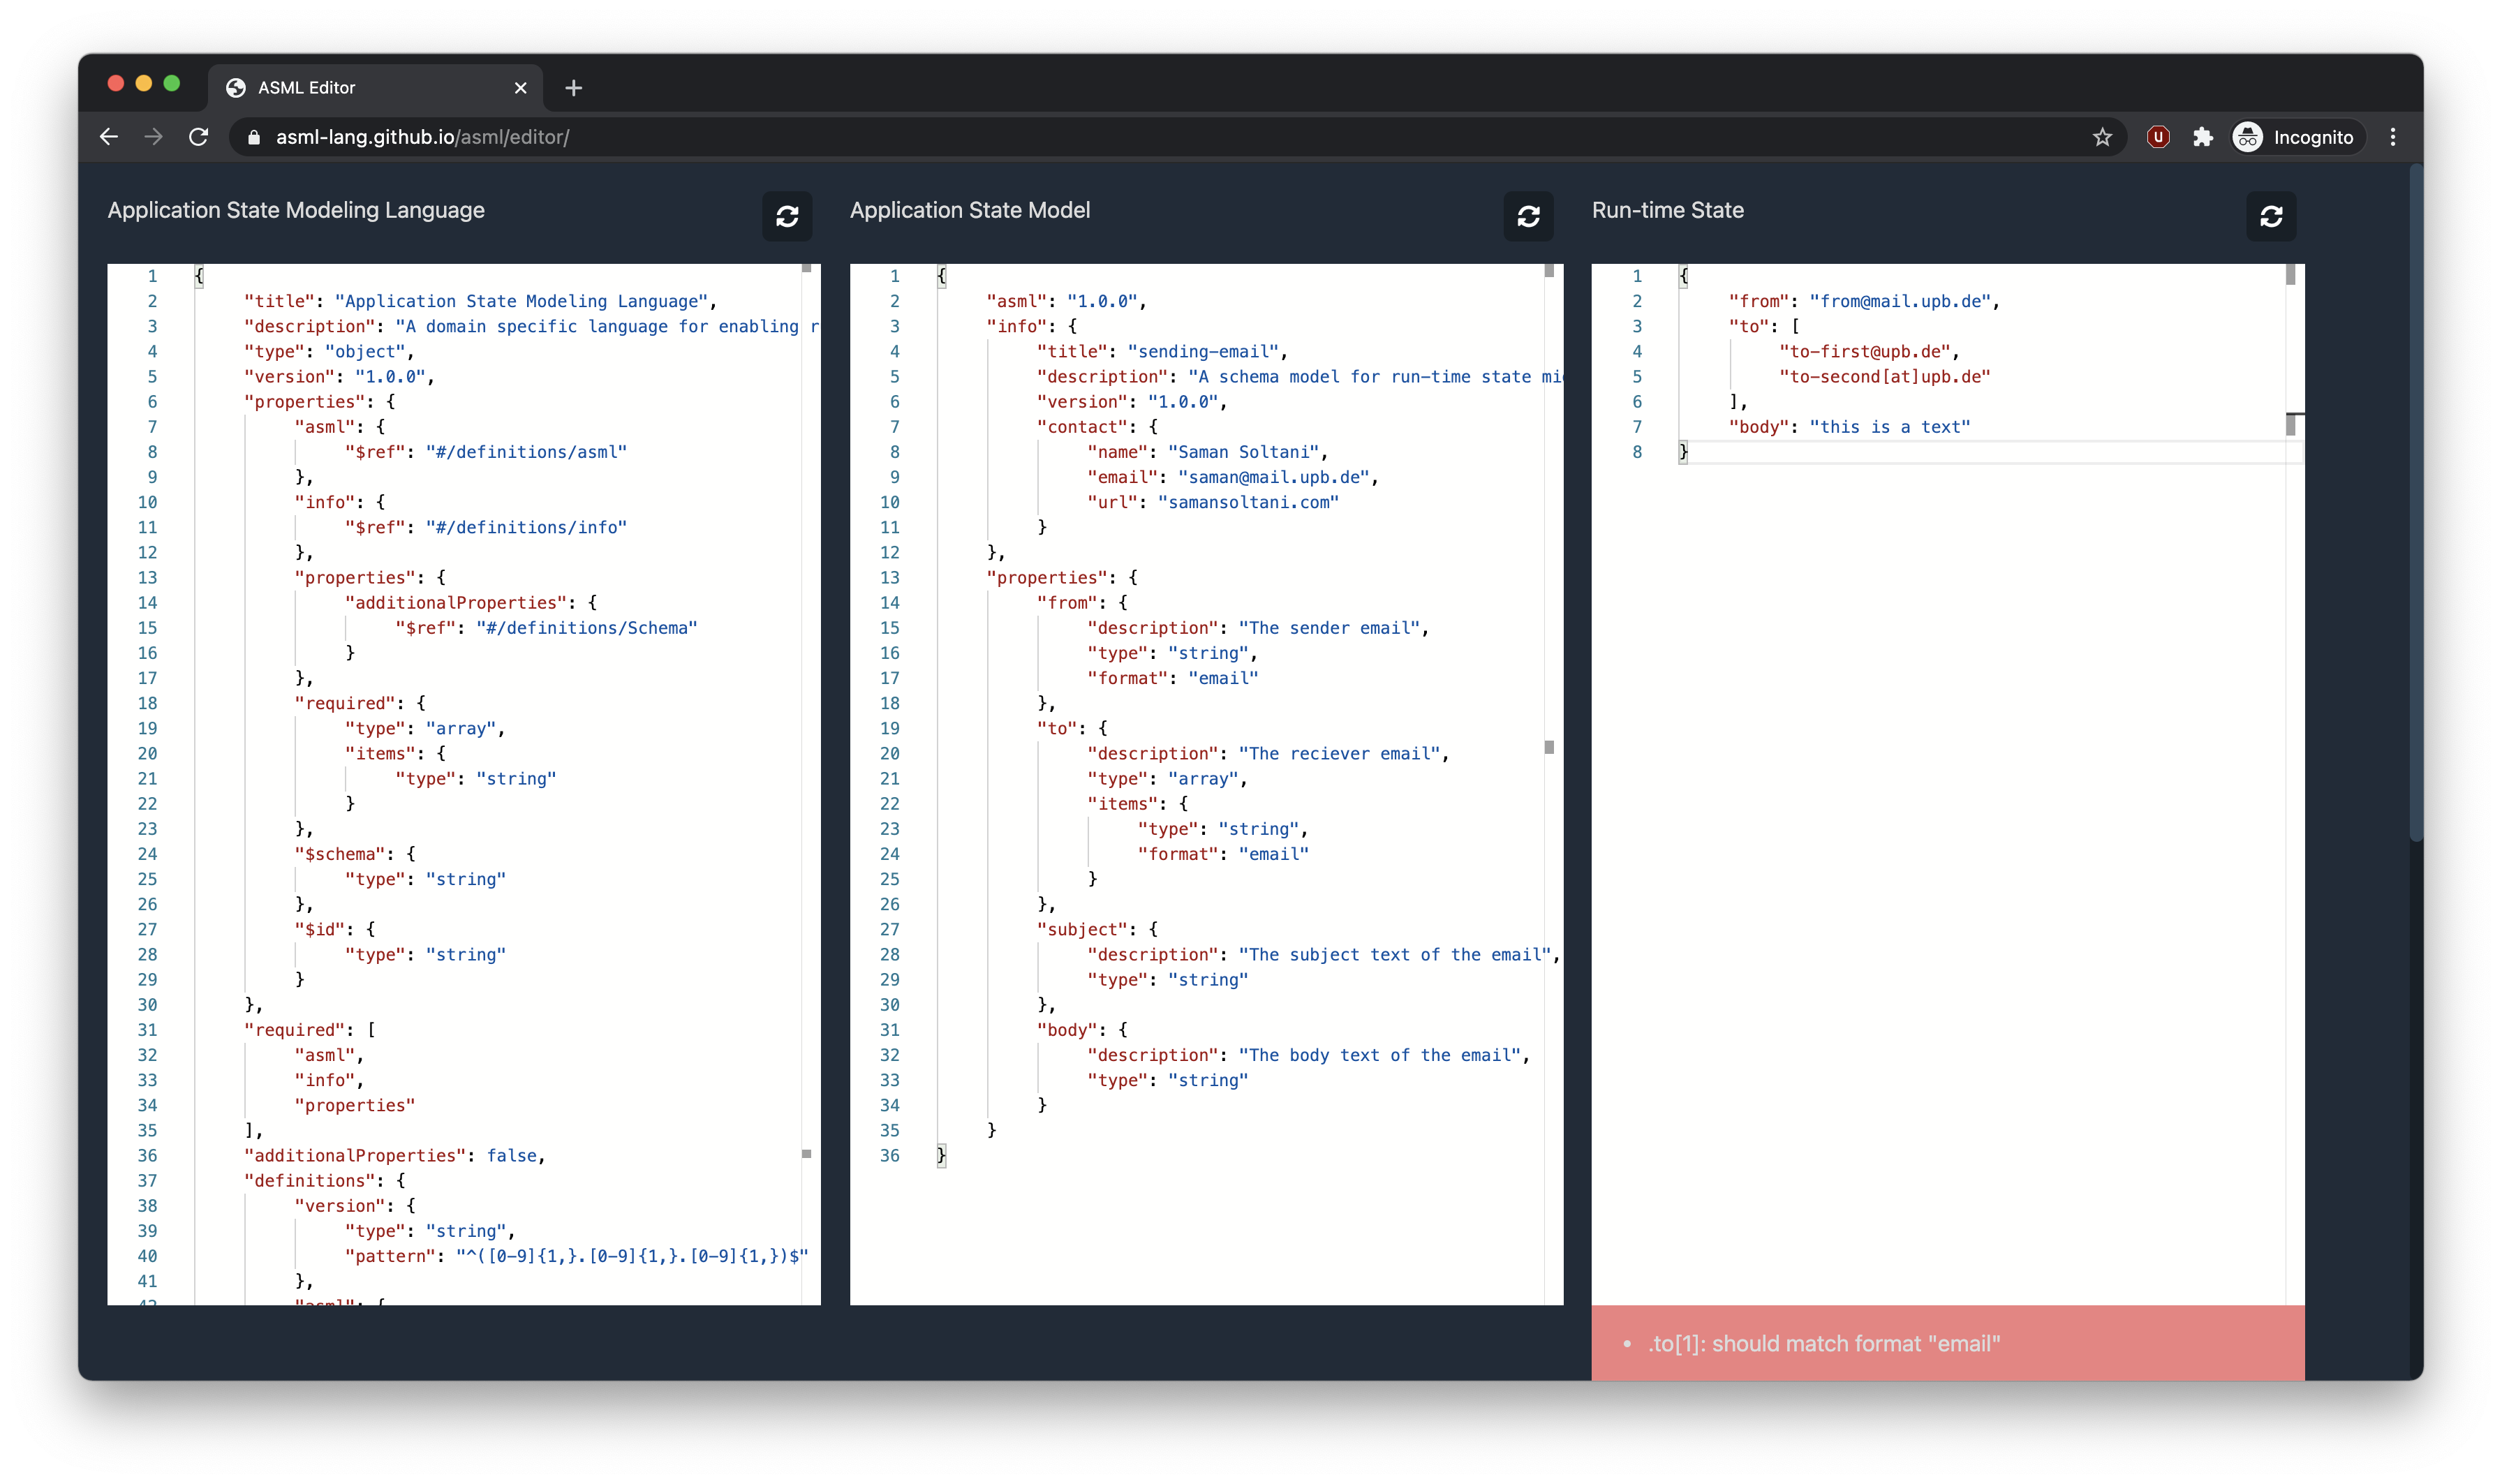
\includegraphics[width=\linewidth]{../figures/asml-editor.png}
    \centering
    \caption{ASML Editor live playground}
    \label{fig:asml-editor}
\end{figure} \FloatBarrier

\subsection{ASML CLI}
ASML CLI is a command-line interface that helps developers to validate Application State Model and generate interfaces based on them for different programming languages. This tool is published on NPM\footnote{\url{https://www.npmjs.com/package/asml-cli}}.

This tool generates data types and some helpers methods for serializing and deserializing the run-time state in JSON. ASML CLI supports code generating in these programming languages:
Ruby, JavaScript, Flow, Rust, Kotlin, Dart, Python, C\#, Go, C++, Java, TypeScript, Swift, Objective-C, Elm.

\subsection{ASML Validator Library}
ASML Validator is a JavaScript library that allows a JavaScript application to validate the Application State Model and Run-time State against Application State Modeling Language. This library using ASML Schema Library as the main schema for validating. The source code of this library is available on GitHub\footnote{\url{https://github.com/asml-lang/asml-validator}}. Also, this library is published on NPM\footnote{\url{https://www.npmjs.com/package/asml-validator}}, and it is used in Run-time State Migration JavaScript Library, ASML Editor, and ASML CLI.

